\section{Zeilsetzung}
In diesem Versuch soll die thermische Elektronenemission ("Glühelektrischer Effekt") untersucht werden. Insbesondere soll hier die
Temperaturabhängigkeit und die Austrittsarbeit des verwendeten Wolframs mit Hilfe der Kennlinien untersucht werden.

\section{Theorie}
Als glühelektrischer Effekt wird die Emission von Elektronen von einem aufgeheizten Metall bezeichnet. Hierzu müssen sie Elektronen eine
Austrittsarbeit verrichten. Diese Austrittsarbeit lässt sich an dem Modell eines Potentialtopfes erklären. Das Elektron ist in dem
Potentialtopf des positiv geladenen Atomgitters gebunden und es muss die Austrittsarbeit leisten, um aus diesem Potential herauszugelangen.

Dieser Versuch muss in einer Hochvakuumdiode durchgeführt werden, damit die freigesetzten Elektronen nicht mit der Umgebungsluft reagieren.
Der schematische Aufbau einer Hochvakuumdiode ist in Abbildung \ref{abb:1} dargestellt.

\begin{figure}
  \centering
  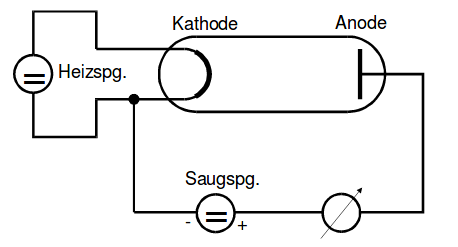
\includegraphics[scale = 0.5]{Hochvakuumdiode.png}
  \caption{Schematischer Aufbau einer Hochvakuumdiode. \cite{Q1}}
  \label{abb:1}
\end{figure}

Die Heizspannung sorgt für die Erhitzung des Metalles in der Kathode, hier Wolfram. Die Elektronen treten aus der Kathode aus
und werden durch die Beschleunigungsspannung in Richtung der Anode beschleunigt. Der gemessene Strom zwischen Anode und Kathode ist proportional
zu den herausgelösten Elektronen. Wenn der Strom $I$ in Abhängigkeit von der Beschleunigungsspannung $U$ aufgetragen wird, es entsteht eine typische
Kennlinie (Abbildung \ref{abb:2}).

\begin{figure}
  \centering
  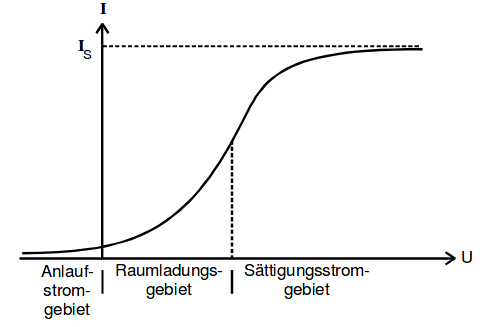
\includegraphics[scale = 0.5]{Kennlinie.png}
  \caption{Kennlinie. \cite{Q1}}
  \label{abb:2}
\end{figure}

Diese Kennlinie ist in drei Bereiche unterteilt, die jeweils durch ein Gesetz beschrieben werden.
Der erste Bereich wird als \textbf{Anlaufstromgebiet} bezeichnet, hier ist die Beschleunigungsspannung negativ, sie kann also eher als Gegenspannung
verstanden werden. Dieser Strom lässt sich darauf zurückführen, dass die aus der Kathode austretenden Elektronen eine statistisch verteilte
kinetische Energie haben. Es existieren also endlich viele Elektronen, die trotz Gegenspannung die Anode erreichen. Die Stomdichte $j$ in
Abhängigkeit des Gegenstroms $U$ und der Temperatur $T$ ist gegeben durch

\begin{equation}
  j(V) = A \cdot exp \left(- \frac{e_0 V}{k_B T} \right)
\end{equation}

wobei $A$ eine Konstante, $e_0$ die Elementarladung und $k_B$ die Boltzmannkonstante darstellt.

Das \textbf{Raumladungsgebiet} wird durch das \textbf{Langmuir-Schottkysche Raumladungsgesetz} beschrieben

\begin{equation}
  j(V) = \frac{4}{9} e_0 \sqrt{\frac{2e_0}{m_o}} \frac{V^{3/2}}{a^2},
\end{equation}

wobei $a$ der Abstand zwischen Anode und Kathode und $m_0$ die Elektronenmasse beschreibt. Hierbei werden Elektronen aus dem Metall durch den Glühelektrischen Effekt herausgelöst und in Richtung der Anode beschleunigt.
Der gemessene Strom $I$ ist dabei proportional zu $V^{3/2}$.

Der letzte Abschnitt der Kennlinie wird durch das \textbf{Sättigungsstromgebiet} charakterisiert. Hier nähert sich der Strom einem
Sättigungswert an. Dies ist darauf zurückzuführen, dass die freigewordenen Elektronen zwischen der Kathode und der Anode ein
eigenes elektrisches Gegenfeld erzeugen. Bei einer bestimmten Spannung ist das Gegenfeld der Elektronen genauso groß wie das
eigentlich durch die Beschleunigungsspannung erzeugte elektrische Feld. Somit stellt sich ein Gleichgewicht ein und der Strom $I$
kann nicht mehr größer werden. Dieser Bereich wird durch die folgende \textbf{Richardson Gleichung} beschrieben, mit $\phi$ die Austrittsarbeit beschreibt,

\begin{equation}
  j_s(T) = 4 \pi T^2 \frac{e_0 m_0 k^2}{h^3} exp \left(- \frac{e_0 \phi}{k_B T} \right)
\end{equation}

\section{Durchführung}
Zunächst wird der Versuchsaufbau nach dem Schaltplan aufgebut (siehe Abbildung \ref{abb:3}).

\begin{figure}
  \centering
  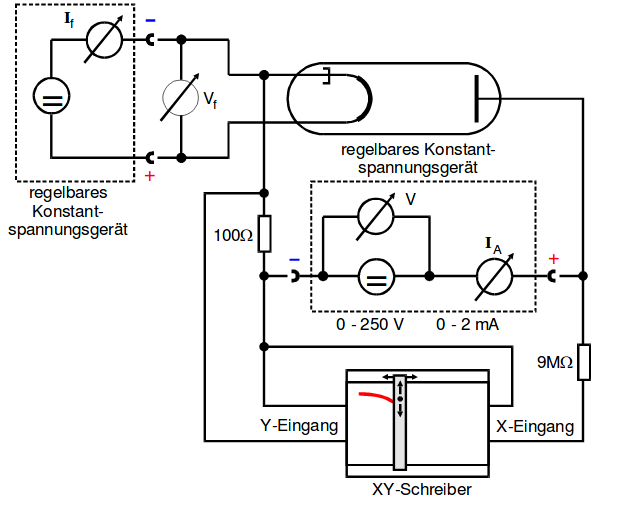
\includegraphics[scale = 0.5]{Aufbau.png}
  \caption{Aufbau. \cite{Q1}}
  \label{abb:3}
\end{figure}

Es werden zunächst 4 Messungen des Sättigungsbereiches durchgeführt mit jeweils verschiedenen Heizspannungen zwischen \SI{1,8}{\ampere} und
\SI{2,3}{\ampere}. Dabei werden zu ungefähr 20 verschiedenen Beschleunigungsspannungen (im Bereich von \SI{0}{\volt} bis \SI{250}{\volt}) die Stromstärken $I$ gemessen.

Zur Messung des Raumladungsgebietes wird die maximale Stromstärke von \SI{2,3}{\ampere} eingestellt und etwa 50 Messpaare genommen, hierbei
soll vor allem im Bereich bis \SI{100}{\volt}, um den Raumladungsbereich gut darzustellen.

Bei der Messung des Anlaufstromgebietes wird ein Nanoamperemeter und ein externes Voltmeter angeschlossen, um die geringen Stromstärken
genauer messen zu können. Hier werden möglichst viele Messwerte aufgenommen, hier sind etwa 20.
